%%%%%%%%%%%%%%%%%%%%%%%%%%%%%%%%%%%%%%%%%
% Stylish Article
% LaTeX Template
% Version 2.2 (2020-10-22)
%
% This template has been downloaded from:
% http://www.LaTeXTemplates.com
%
% Original author:
% Mathias Legrand (legrand.mathias@gmail.com) 
% With extensive modifications by:
% Vel (vel@latextemplates.com)
% Jacqueline Näther (jnaether@uni-osnabrueck.com)
% Fabian Imkenberg (fimkenberg@uni-osnabrueck.com)
%
% License:
% CC BY-NC-SA 3.0 (http://creativecommons.org/licenses/by-nc-sa/3.0/)
%
%%%%%%%%%%%%%%%%%%%%%%%%%%%%%%%%%%%%%%%%%

%----------------------------------------------------------------------------------------
%	PACKAGES AND OTHER DOCUMENT CONFIGURATIONS
%----------------------------------------------------------------------------------------

\documentclass[fleqn,10pt]{SelfArx} % Document font size and equations flushed left

\usepackage[english]{babel} % Specify a different language here - english by default

\usepackage{lipsum} % Required to insert dummy text. To be removed otherwise

\usepackage[nolist]{acronym}	% [nolist]: Acronym list should not be print out.

\usepackage{listings}	% Required to insert lstlisting environment for code.

\usepackage{makecell}	% For manual line breaks in tables

\usepackage{caption}
\usepackage{subcaption}	% Needed for subfigures

%----------------------------------------------------------------------------------------
%	COLUMNS
%----------------------------------------------------------------------------------------

\setlength{\columnsep}{0.55cm} % Distance between the two columns of text
\setlength{\fboxrule}{0.75pt} % Width of the border around the abstract

%----------------------------------------------------------------------------------------
%	COLORS
%----------------------------------------------------------------------------------------

\definecolor{color1}{RGB}{172,06,52} % Corporate Design Colour of University of Osnabrueck
\definecolor{color2}{RGB}{207,208,209} % Corporate Design Colour of University of Osnabrueck
\definecolor{color3}{RGB}{251,185,0} % Corporate Design Colour of University of Osnabrueck
\definecolor{codegreen}{rgb}{0,0.6,0}
\definecolor{codegray}{rgb}{0.5,0.5,0.5}
\definecolor{codepurple}{rgb}{0.58,0,0.82}
\definecolor{backcolour}{rgb}{0.95,0.95,0.92}

%----------------------------------------------------------------------------------------
%	LISTING STYLE
%----------------------------------------------------------------------------------------

\lstdefinestyle{mystyle}{
    backgroundcolor=\color{backcolour},   
    commentstyle=\color{codegreen},
    keywordstyle=\color{magenta},
    numberstyle=\tiny\color{codegray},
    stringstyle=\color{codepurple},
    basicstyle=\ttfamily\footnotesize,
    breakatwhitespace=false,         
    breaklines=true,                 
    captionpos=b,                    
    keepspaces=true,                 
    numbers=left,                    
    numbersep=5pt,                  
    showspaces=false,                
    showstringspaces=false,
    showtabs=false,                  
    tabsize=2
}

\lstset{style=mystyle}

%----------------------------------------------------------------------------------------
%	HYPERLINKS
%----------------------------------------------------------------------------------------

\usepackage{hyperref} % Required for hyperlinks

\hypersetup{
	hidelinks,
	colorlinks,
	breaklinks=true,
	urlcolor=color3,
	citecolor=color1,
	linkcolor=color1,
	bookmarksopen=false,
	pdftitle={Title},
	pdfauthor={Author},
}

%----------------------------------------------------------------------------------------
%	ARTICLE INFORMATION
%----------------------------------------------------------------------------------------

\JournalInfo{
\includegraphics[width=0.3\linewidth]{logo_uni}}
\Archive{} %!!NEEDED, otherwise \tableofcontent error, is for Additional notes below university logo (e.g. copyright, DOI, review/research article)

\PaperTitle{Reimplementation of a Cycle-Consistent Adversarial Network for unpaired Image-to-Image Translation}

\Authors{Fabian Imkenberg, Jacqueline Naether}

\Keywords{CycleGAN --- Unpaired Image-to-Image Translation --- CycleWGAN -- Regularized CycleGAN} 
\newcommand{\keywordname}{Keywords} % Defines the keywords heading name

%----------------------------------------------------------------------------------------
%	ABSTRACT
%----------------------------------------------------------------------------------------

\Abstract{In this project, we reimplement the paper "Unpaired Image-to-Image Translation using Cycle-Consistent Adversarial Networks" and test its performance with three different datasets, from which two were given by the paper and another new one. After reimplementation of the Cycle \ac{GAN} with minor justified changes, two modifications are applied. This results in the three different variations of Cycle\ac{GAN}s, Classical Cycle\ac{GAN}, Regularized Cycle\ac{GAN}, Cycle \ac{WGAN}. After the implementation follows the analysis of the performance of the different \ac{GAN} variations and the different datasets. Here it becomes clear that the Cycle\ac{GAN} already shows progress after a few training steps, whereas changing colours through the Cycle\ac{GAN} is learned much faster and easier than learning more complicated features such as eyes.}

%----------------------------------------------------------------------------------------

\begin{document}
\maketitle
\tableofcontents
\thispagestyle{empty} % Removes page numbering from the first page

%----------------------------------------------------------------------------------------
%	ARTICLE CONTENTS
%----------------------------------------------------------------------------------------

\section*{Introduction}
\addcontentsline{toc}{section}{Introduction}
As the basis of this project, the paper \textit{Unpaired Image-to-Image Translation using Cycle-Consistent Adversarial Networks} from the \ac{BAIR} laboratory is studied. The aim of the paper is to change different information in images. The developed network creates a generated image based on an existing input image. Three different datasets for image generation are presented in this paper. A translation from a photo to a painting by Monet, from zebras to horses, and from summer to winter and vice versa in each case. The paper complements what has been learned in the module \ac{IANNWTF} by two essential building blocks that are basically interdependent.~\cite{image-to-image-ccan}

Until now, training data was mostly available in input-output pairs. If one takes the translation from summer to winter as an example, this means that for every photo of a location in summer, there also exists a photo of the same location in winter. Thus, the network would learn the translation based on one-to-one examples. In contrast, in case of the paper, the network is trained based on two domains. So, the network learns the different properties of summer and winter based on random images belonging to one of the two domains. As a side effect, this significantly facilitates the acquisition of suitable datasets, since no direct correlation between the images of the two domains is necessary.~\cite{image-to-image-ccan}

The second building block, the \ac{GAN} as introduced in \ac{IANNWTF}, is extended to a so called Cycle\ac{GAN}. The name is motivated by the use of cycle consistency loss in the training phase.

In this paper, the Cycle\ac{GAN} architecture (based on~\cite{image-to-image-ccan}) will be reimplemented and tested to obtain a more in-depth understanding of its benefits and drawbacks. Additionally, different variations of the classical Cycle\ac{GAN} are analyzed and their performances on different datasets compared.

%------------------------------------------------

\section{Methodology}

The architecture described in this paper should be based on the classical Cycle\ac{GAN} approach, but must also enable some modifications for the implementation of variations. So, it has to work for different datasets and needs to have a well-organized structure that allows the architecture to be modified while maintaining a clear and understandable network design. Therefore, amomg other things, the methodological basics of the architecture from the paper have to be worked out. In the following, these basics will be explained.

\subsection{Related approaches}
First, an overview of related work for this paper is provided.

\paragraph{\acl{GAN}s} basically consist of two neural networks which more or less compete with each other, the \textit{Generator} and the \textit{Discriminator}. The generator takes the input, often provided in form of an encoding, and generates a fake image from it, while the discriminator tries to discriminate between generated and real images. Both parts of the network are trained individually from each other. The loss used in training is the adversarial loss.~\cite{Introduction-to-Cycle-GANs, GAN-Courseware}

\paragraph{Cycle\ac{GAN}s} extend this concept, in terms of unpaired image-to-image translation. As mentioned in the introduction, the chosen paper uses domains of input images \textit{D\textsubscript{x}} and output images \textit{D\textsubscript{y}}. The Generator is trained by two main functions: Generating images from domain \textit{D\textsubscript{x}} to images from domain \textit{D\textsubscript{y}} ($G: X \rightarrow Y$) and vice versa ($F: Y \rightarrow X$). This principle is shown in \autoref{fig:mappingFunctions}.~\cite{image-to-image-ccan}

\begin{figure} \centering 
% Using \begin{figure*} makes the figure take up the entire width of the page
	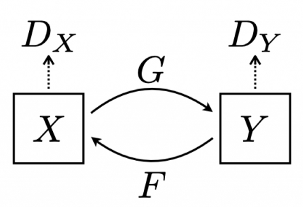
\includegraphics[width=0.8\linewidth]{mappingFunctions}
	\caption{Mapping functions of the Cycle\ac{GAN}~\cite{image-to-image-ccan}}
	\label{fig:mappingFunctions}
\end{figure}

From this, it can be inferred that a simple for- and backward translation may result in a back-translation that does not correspond to the original input image, but to a different image within the input image domain. To address this issue, cycle consistency loss is introduced. It is used in addition to the adversarial loss so that the network learns to return to the original image after a for- and backward translation. The cycle consistency losses for the two mapping functions are shown in the \autoref{fig:cycleConsistencyLoss}.~\cite{image-to-image-ccan}

\begin{figure*}[htb] \centering 
% Using \begin{figure*} makes the figure take up the entire width of the page
	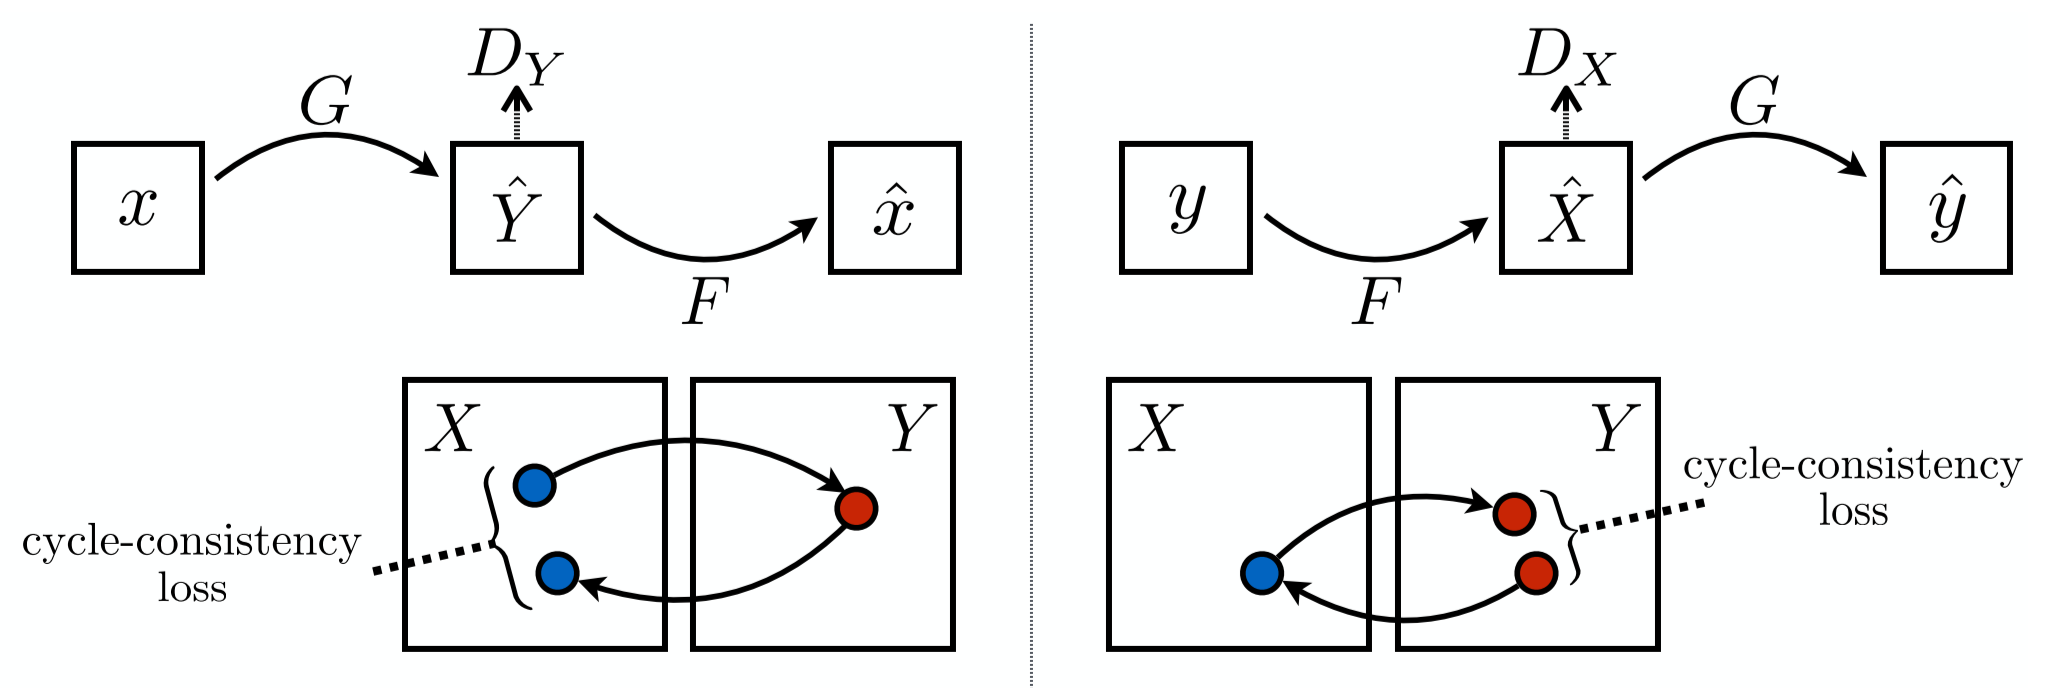
\includegraphics[width=\linewidth]{cycleConsistencyLoss}
	\caption{Cycle Consistency Losses in the for- and backward translation~\cite{image-to-image-ccan}}
	\label{fig:cycleConsistencyLoss}
\end{figure*}

\paragraph{Cycle Wasserstein\ac{GAN}s} are an improvement of the classical Cycle\ac{GAN}. This type was introduced due to the frequent training instabilites of Cycle\ac{GAN}s. CycleW\ac{GAN}s aim to overcome this issue by introducing the Wasserstein distance which has better continuity and differentiability properties in contrast to local saturated loss functions. Thus, the approach is intended to reduce the problem of vanishing gradients.~\cite{wgan-improvement}.

\subsection{Formulation}
For a better understanding of the function and the subsequent implementation of the losses, the mathematical background is explained in more detail.

\paragraph{Adversarial Loss} is already used in the training of a \ac{GAN}s. It arises from the fact that the generator \textit{G} and discriminator \textit{D} compete with each other. If the generator generates particularly good fake images which the discriminator can no longer identify as such, the discriminator's loss automatically increases. On the other hand, the loss of the generator decreases. This behaviour is the same the other way round. It is mathematically described in \cite{Source-GAN} as follows:
\begin{equation*}
\begin{split}
\min_{G} \max_{D} V(D,G) =&~\mathbb E_{x \sim p_{data}(x)} [\log D(x)] \\\
&+ \mathbb E_{z \sim p_{z}(z)} [\log (1-D(G(z)))]
\end{split}
\end{equation*}

\paragraph{Cycle Consistency Loss} is used in addition to the adversarial loss in the Cycle\ac{GAN}. As briefly explained before, a generator \textit{G} translates an image \textit{Input\_ A} from domain \textit{X} to an image \textit{B} from domain \textit{Y}. In the backward translation of the generator \textit{F}, an image \textit{Cyclic\_ A} from domain \textit{X} will be created using image \textit{B} from domain \textit{Y}. The difference between image \textit{Input\_ A} and \textit{Cyclic\_ A} forms the cycle consistency loss \cite{Introduction-to-Cycle-GANs}. In \cite{Introduction-to-Cycle-GANs}, the cycle consistency loss is mathematically described as follows:
\begin{equation*}
	Loss_{cyc}(G,F,X,Y) = \frac{1}{m} \sum^{m}_{i=1}[F(G(x_i))-x_i]+[G(F(y_i))-y_i]
\end{equation*}

In summary, the Cycle\ac{GAN} is composed of two generators, \textit{Generator A2B} and \textit{Generator B2A}, as well as two discriminators, \textit{Discriminator A} and \textit{Discriminator B}. This architecture is shown in simplified form in \autoref{fig:simplified-cycle-gan}.

\begin{figure}[htb] 
	\centering 
	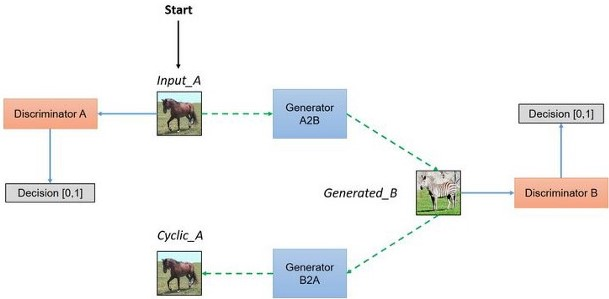
\includegraphics[width=\linewidth]{simplified-cycle-gan}
	\caption{A simplified architecture of a Cycle\ac{GAN} \cite{Introduction-to-Cycle-GANs}}
	\label{fig:simplified-cycle-gan}
\end{figure}

\paragraph{Identity Loss} is also introduced in paper \cite{image-to-image-ccan}. The loss can be seen as a regularization technique for encouraging the generator to preserve the color composition between the input- and the output image. This is done by providing the generator real images from the target domain, with the goal to not translate them. Mathematically, the identity loss is defined as follows \cite{image-to-image-ccan}:
\begin{equation*}
\begin{split}
	Loss_{identity}(G,F) =&~\mathbb E_{y \sim p_{data}(y)}[||G(y) - y||_1] \\\
&+ \mathbb E_{x \sim p_{data}(x)}[||F(x)-x||_1]
\end{split}
\end{equation*}

\subsection{Datasets}
In addition to the architecture, suitable datasets must be selected. These should be versatile and contain images that are suitable for the classification into two domains.

\paragraph{Tensorflow} provides different datasets specifically suited for Cycle\ac{GAN}s including for example apple and orange domains as well as photo and Monet painting domains. These are called \textit{cycle\_gan/apple2orange} and \textit{cycle\_gan/monet2photo}. The datasets are divided into training and test datasets. \autoref{tab:datasetTF} shows the four parts of the standard configuration with the number of examples included in each dataset. Every example consist of image-label pairs.~\cite{google-tf-datasets}

\begin{table}[htb]
\centering
\caption{Structure of the standard configuration split of the Tensorflow datasets \textit{cycle\_gan/apple2orange} and \textit{cycle\_gan/monet2photo}~\cite{google-tf-datasets}}
\label{tab:datasetTF}
\begin{tabular}{c c c}
\textbf{index} & \makecell[cc]{\textbf{examples} \\ \textbf{\texttt{apple2orange}}} & \makecell[cc]{\textbf{examples} \\ \textbf{\texttt{monet2photo}}}\\ \hline
'testA' & 266 & 121 \\ \hline
'testB' & 248 & 751 \\ \hline
'trainA' & 995 & 1072 \\ \hline
'trainB' & 1019 & 6287 \\ \hline
\end{tabular}
\end{table}

\paragraph{Kaggle} provides another dataset called \textit{arnaud58/selfie2anime}. This one is selected to analyze the performance of the Cycle\ac{GAN} on a dataset which was not part of the classical Cycle\ac{GAN} paper~\cite{image-to-image-ccan}. It contains images of animes and women selfies. The number of examples included in this dataset are shown in \autoref{tab:datasetKaggle}. \cite{kaggle-dataset}

\begin{table}[htb]
\centering
\caption{Structure of the standard configuration split of the Kaggle dataset \textit{arnaud58/selfie2anime}~\cite{kaggle-dataset}}
\label{tab:datasetKaggle}
\begin{tabular}{c c}
\textbf{index} & \makecell{\textbf{examples} \\ \textbf{\texttt{selfie2anime}}} \\ \hline
'testA' & 100 \\ \hline
'testB' & 100 \\ \hline
'trainA' & 3400 \\ \hline
'trainB' & 3400 \\ \hline
\end{tabular}
\end{table}
%------------------------------------------------
\section{Implementation}
The implementation is performed using the taught three steps from the module \ac{IANNWTF}: pre-processing, training and test~\cite{implementingANsCourseware02, implementingANsCourseware03}. In addition, the methods mentioned in the section before are used to develop the Cycle\ac{GAN} architecture. Furthermore, functions of the Tensorflow and Keras libraries are utilized in nearly every part of the implementation. The realization of the implementation and usage of the different libraries is now explained in more detail.

\subsection{Network Architecture}
The architecture is built as explained in the section before. A class \texttt{Cycle\_GAN\_Generator} and a class \texttt{Cycle\_GAN\_ Discriminator} are implemented. In the following, two instances of each class are created, \texttt{generator\_A\_to\_B} and \texttt{generator\_B\_to\_A} as well as \texttt{discriminator\_A} and \texttt{discriminator\_B}.

\paragraph{Generator Class} inherits from the Keras class \texttt{Layer}. In general, the class is build up of three parts, the \textit{Encoding}, the \textit{Transformation} and the \textit{Decoding}. Each part again consists of different layers. The structure of the generator is shown in \autoref{fig:generator}.~\cite{Introduction-to-Cycle-GANs}

\begin{figure*}[htb] 
	\centering 
	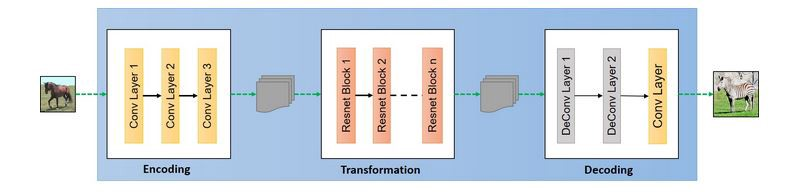
\includegraphics[width=\linewidth]{generator}
	\caption{The high-level structure of the Cycle\ac{GAN}'s generator \cite{Introduction-to-Cycle-GANs}}
	\label{fig:generator}
\end{figure*}

The \textbf{Encoding} extracts the features of the original input image. In \texttt{Cycle\_GAN\_Generator}, the encoding consists of exactly three convolutional layers, as depicted in \autoref{fig:generator}. The Keras class \texttt{Conv2D} is used for this. As activation function \ac{ReLu} are selected, using the Keras class \texttt{ReLu}. Furthermore, the Keras class \texttt{InstanceNormalization} is utilized to enable this special form of group normalization (see \cite{google-tf-InstanceNormalization} for more details). Instance Normalization is well-suited for the datasets with batch size 1 as recommended by the paper. The filter sizes of each \texttt{Conv2D} layer are quartered to reduce the complexity and enable a faster training of the Cycle\ac{GAN}. All other relevant parameters like \texttt{kernel\_size}, \texttt{strides}, \texttt{activation}, \texttt{padding} and the \texttt{kernel\_initializer} are taken from the paper. The specifications and values for the three \texttt{Conv2D} layers are shown in \autoref{tab:encoderValues}.~\cite{image-to-image-ccan}

\begin{table}[htb]
\centering
\caption{Values of the convolutional layer specifications in the encoding part of the class \texttt{Cycle\_GAN\_Generator}~\cite{image-to-image-ccan}.}
\label{tab:encoderValues}
\begin{tabular}{c c c c}
\textbf{variable} & \makecell[cc]{\textbf{\texttt{Conv2D}} \\ \textbf{\texttt{Layer 1}}} & \makecell[cc]{\textbf{\texttt{Conv2D}} \\ \textbf{\texttt{Layer 2}}} & \makecell[cc]{\textbf{\texttt{Conv2D}} \\ \textbf{\texttt{Layer 3}}} \\ \hline
\textbf{\texttt{filters}} & 16 & 32 & 64 \\ \hline
\textbf{\texttt{kernel\_size}} & (7,7) & (3,3) & 3,3) \\ \hline
\textbf{\texttt{strides}} & (1,1) &  (2,2) & (2,2) \\ \hline
\textbf{\texttt{activation}} & None & None & None \\ \hline 
\textbf{\texttt{padding}} & "same" & "same" & "same" \\ \hline
\makecell[cc]{\textbf{\texttt{kernel\_}} \\ \textbf{\texttt{initializer}}} & \makecell[cc]{\texttt{Random} \\ \texttt{Normal}} & \makecell[cc]{\texttt{Random} \\ \texttt{Normal}} & \makecell[cc]{\texttt{Random} \\ \texttt{Normal}} \\ \hline
\end{tabular}
\end{table}

The \textbf{Transformation} is needed to relate closely spaced features extracted from the input image by the previous encoding \cite{Introduction-to-Cycle-GANs}. And this is exactly what the blocks of \acp{ResNet}, like shown in \autoref{fig:generator}, are needed for. Every \ac{ResNet} is build up by two \texttt{Conv2D} layers, two layers of \texttt{InstanceNormalization}, a \ac{ReLu} activation layer and a layer \texttt{Concatenate}, which is also a Keras class. A new class \texttt{ResNet\_Block}, which also inherits from the Keras class \texttt{Layer}, is implemented. All values for the layers are taken from the paper. The convolutional layer specifications are shown in \autoref{tab:transformerValues}.

\begin{table}[htb]
\centering
\caption{Values of the convolutional layer specifications in the \ac{ResNet} block (part of the transformation part of the class \texttt{Cycle\_GAN\_Generator}~\cite{image-to-image-ccan}.}
\label{tab:transformerValues}
\begin{tabular}{c c c}
\textbf{variable} & \makecell[cc]{\textbf{\texttt{Conv2D}} \\ \textbf{\texttt{Layer 1}}} & \makecell[cc]{\textbf{\texttt{Conv2D}} \\ \textbf{\texttt{Layer 2}}} \\ \hline
\textbf{\texttt{filters}} & 256 & 256 \\ \hline
\textbf{\texttt{kernel\_size}} & (3,3) & (3,3) \\ \hline
\textbf{\texttt{strides}} & (1,1) &  (1,1) \\ \hline
\textbf{\texttt{activation}} & None & None \\ \hline 
\textbf{\texttt{padding}} & "same" & "same" \\ \hline
\makecell[cc]{\textbf{\texttt{kernel\_}} \\ \textbf{\texttt{initializer}}} & \makecell[cc]{\texttt{Random} \\ \texttt{Normal}} & \makecell[cc]{\texttt{Random} \\ \texttt{Normal}} \\ \hline
\end{tabular}
\end{table}

Instances of this class are created as a layer in the class \texttt{Cycle\_GAN\_Generator}. The number of instances depends on the instance variable \texttt{n\_resnet}, which is set to six by default. Six \ac{ResNet} blocks are used if the image size is \textit{128~x~128}, nine blocks are use for an image size of \textit{256~x~256} or higher~\cite{image-to-image-ccan}.

The \textbf{Decoding} now leads back to an output image. For this, the low-level features are worked out with the help of the transpose convolution, see \cite{Introduction-to-Cycle-GANs}. To achieve this, the Keras class \texttt{Conv2DTranspose} is used in this part. Finally, as shown in \autoref{fig:generator}, another \texttt{Conv2D} is used, in conjunction with an activation function of the Keras class \texttt{tanh}. The values of the transposed convolution layer specifications is found in \autoref{tab:decoderValues1}, for the convolutional layer specifications in \autoref{tab:decoderValues2}.

\begin{table}[htb]
\centering
\caption{Values of the transposed convolutional layer specifications in the decoding part of the class \texttt{Cycle\_GAN\_Generator}~\cite{image-to-image-ccan}.}
\label{tab:decoderValues1}
\begin{tabular}{c c c}
\textbf{variable} & \makecell[cc]{\textbf{\texttt{Conv2D}} \\ \textbf{\texttt{Transpose}} \\ \textbf{\texttt{Layer 1}}} & \makecell[cc]{\textbf{\texttt{Conv2D}} \\ \textbf{\texttt{Transpose}} \\ \textbf{\texttt{Layer 2}}} \\ \hline
\textbf{\texttt{filters}} & 32 & 16 \\ \hline
\textbf{\texttt{kernel\_size}} & (3,3) & (3,3)  \\ \hline
\textbf{\texttt{strides}} & (2,2) & (2,2)  \\ \hline
\textbf{\texttt{activation}} & None & None  \\ \hline 
\textbf{\texttt{padding}} & "same" & "same" \\ \hline
\makecell[cc]{\textbf{\texttt{kernel\_}} \\ \textbf{\texttt{initializer}}} & \makecell[cc]{\texttt{Random} \\ \texttt{Normal}} & \makecell[cc]{\texttt{Random} \\ \texttt{Normal}}  \\ \hline
\end{tabular}
\end{table}

\begin{table}[htb]
\centering
\caption{Values of the convolutional layer specifications in the decoding part of the class \texttt{Cycle\_GAN\_Generator}~\cite{image-to-image-ccan}.}
\label{tab:decoderValues2}
\begin{tabular}{c c}
\textbf{variable} & \makecell[cc]{\textbf{\texttt{Conv2D}} \\ \textbf{\texttt{Layer 4}}} \\ \hline
\textbf{\texttt{filters}} & 3 \\ \hline
\textbf{\texttt{kernel\_size}} & (7,7) \\ \hline
\textbf{\texttt{strides}} & (1,1) \\ \hline
\textbf{\texttt{activation}} & None \\ \hline 
\textbf{\texttt{padding}} & "same" \\ \hline
\makecell[cc]{\textbf{\texttt{kernel\_}} \\ \textbf{\texttt{initializer}}} & \makecell[cc]{\texttt{Random} \\ \texttt{Normal}} \\ \hline
\end{tabular}
\end{table}

\paragraph{Discriminator Class} also inherits from the Keras class \texttt{La- yer}. In this reimplementation the class isn't a simple discriminator class, but a so called \textit{Patch\ac{GAN}}. This one is made up to not only output a single value, but a one-channel feature map of predictions. In this case the output refers to a \textit{70~x~70} receptive field of the original input. Since it has an image as input and a decision vector as output, \texttt{Conv2D} layers, are associated with \texttt{InstanceNormalization} and the activation function \texttt{LeakyReLu}. The values for the layers and there specifications are taken from the paper and are shown in \autoref{tab:discriminatorValues}. The original \texttt{filters} size here again is divided by four in the reimplementation to reduce training time. After first convolutional layer they didn't deliberately used \texttt{InstanceNormalization}. Last layer is a convolution to produce an output of 1-dimension. The structure of the discriminator is also shown in \autoref{fig:discriminator}. \cite{Introduction-to-Cycle-GANs}
\begin{table}[htb]
\centering
\caption{Values of the convolutional layer specifications in the discriminator class \texttt{Cycle\_GAN\_Discriminator}\cite{image-to-image-ccan}.}
\label{tab:discriminatorValues}
\begin{tabular}{c c c c}
\textbf{variable} & \makecell[cc]{\textbf{\texttt{Conv2D}} \\ \textbf{\texttt{Layer 1}}} & \makecell[cc]{\textbf{\texttt{Conv2D}} \\ \textbf{\texttt{Layer 2}}} & \makecell[cc]{\textbf{\texttt{Conv2D}} \\ \textbf{\texttt{Layer 3}}} \\ \hline
\textbf{\texttt{filters}} & 16 & 32 & 64 \\ \hline
\textbf{\texttt{kernel\_size}} & (4,4) & (4,4) & (4,4) \\ \hline
\textbf{\texttt{strides}} & (2,2) & (2,2) & (2,2) \\ \hline
\textbf{\texttt{activation}} & None & None & None\\ \hline 
\textbf{\texttt{padding}} & "same" & "same" & "same" \\ \hline
\makecell[cc]{\textbf{\texttt{kernel\_}} \\ \textbf{\texttt{initializer}}} & \makecell[cc]{\texttt{Random} \\ \texttt{Normal}} & \makecell[cc]{\texttt{Random} \\ \texttt{Normal}} & \makecell[cc]{\texttt{Random} \\ \texttt{Normal}} \\ \hline
\end{tabular}

\begin{tabular}{c c c}
\makecell[cc]{\\ \textbf{variable}} & \makecell[cc]{\\ \textbf{\texttt{Conv2D}} \\ \textbf{\texttt{Layer 4}}} & \makecell[cc]{\\ \textbf{\texttt{Conv2D}} \\ \textbf{\texttt{OutputLayer}}} \\ \hline
\textbf{\texttt{filters}} & 128 & 1 \\ \hline
\textbf{\texttt{kernel\_size}} & (4,4) & (4,4) \\ \hline
\textbf{\texttt{strides}} & (2,2) & (1,1) \\ \hline
\textbf{\texttt{activation}} & None & sigmoid \\ \hline 
\textbf{\texttt{padding}} & "same" & "same" \\ \hline
\makecell[cc]{\textbf{\texttt{kernel\_}} \\ \textbf{\texttt{initializer}}} & \makecell[cc]{\texttt{Random} \\ \texttt{Normal}} & \makecell[cc]{\texttt{Random} \\ \texttt{Normal}} \\ \hline
\end{tabular}
\end{table}

\begin{figure*}[htb] 
	\centering 
	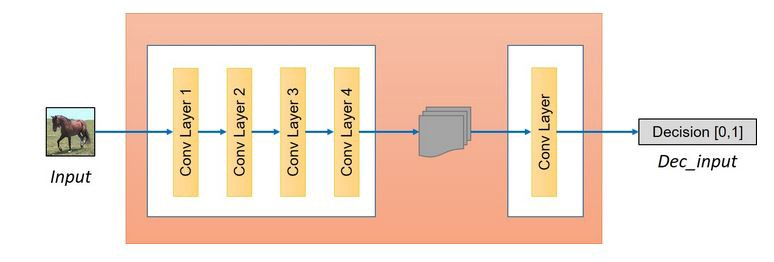
\includegraphics[width=0.8\linewidth]{discriminator}
	\caption{The high-level structure of the Cycle\ac{GAN}'s discriminator \cite{Introduction-to-Cycle-GANs}}
	\label{fig:discriminator}
\end{figure*}

\subsection{Pre-Processing}
In addition to creating the network architecture, the dataset must also be preprocessed. In order to implement easier switching between datasets and comparison versions, in addition to the reimplementation of the paper, different mechanisms were included. For switching between datasets, additional variables (\texttt{is\_selfie2anime\_dataset}, \texttt{is\_ap- ple2orange\_dataset}, \texttt{is\_monet2photo\_dataset}) were implemented to select the dataset to be pre-processed. At the beginning, these variables are used to select which dataset is to be loaded, by setting it \texttt{true}. Only one dataset can be loaded at a time. If several dataset arguments are set to true, the Kaggle dataset is preferred to the Tensorflow datasets due to the \texttt{if-elif-elif} query, and the \textit{apple2orange} dataset is preferred to the \textit{monet2photo} dataset.

Additionally, the dataset size is set to 900 training samples and 100 test samples after pre-processing to have a comparable number of images, between the different datasets. 

Moreover, since two different sources for the three datasets are used, there are a few different steps for pre-processing between the Tensorflow and Kaggle datasets. 

\paragraph{Tensorflow datasets} can be loaded more easily with the \texttt{tfds.load} function from the tensorflow library. In general there is more or less no difference between pre-processing \textit{cylce\_gan/apple2orange} or \textit{cylce\_gan/monet2photo} images. When the dataset is loaded, it is also directly split into test and training data, as well as in two domains for each, and requested as a 2-tuple structure (input, label). To ensure that all images are in the same format and that the training time is not too high, the images are subsequently resized to \textit{128~x~128}. After normalization to a value between $-1$ and $1$ ($2 * (img / 255) - 1$) and reshaping the tensor to \textit{128~x~128~x~3}, the dataset is shuffled and prefetched with a \texttt{buffer\_size} of 128. Batching is omitted, or rather set to one, to facilitate the later definition of real samples in training. All functions used are offered by the Tensorflow library. The values for arguments of the different pre-processing steps are taken directly from the paper.~\cite{image-to-image-ccan}

\paragraph{Kaggle datasets} need a few more pre-processing steps, than Tensorflow ones. The dataset \textit{arnaud58/selfie2anime} is downloaded with Keras function \texttt{image\_dataset\_from\_ directory} and directly batched to one. Because the dataset comes up as one big file, in which the dataset is separated in the different classes mentioned in \autoref{tab:datasetKaggle}, see \cite{kaggle-dataset}, it then needs to be split manually. This is done by using the functions \texttt{take} and \texttt{skip}. Thereupon, the same steps are carried out as for the Tensorflow datasets mentioned before.


\subsection{Training}
Three training epochs are chosen with each epoch having 900 training steps. With these numbers, the training can still be done in a reasonable amount of time. To make the training clearer, various functions have been programmed for different steps in the execution of the program.
 
In the first step the generators are trained. The training starts with taking an image-label pair from domain A and from domain B with the help of the function \texttt{generate\_real\_ dataset}. These pairs are randomly taken from the domains again for each training step. Afterwards the training for the \texttt{generator\_A\_to\_B} takes place and then for the generator \texttt{generator\_B\_to\_A}. Here for, the function \texttt{generator\_train\_step} was programmed, in which the adversarial loss (\texttt{adv\_loss}), the identity loss (\texttt{id\_loss}), the cycle consistency loss for the forward (\texttt{for\_loss}) and backward cycle (\texttt{back\_loss}) and the entire training loss (\texttt{train\_loss}) is computed. The training loss is composed of all other losses as follows:
\begin{equation*}
\begin{split}
train\_loss = &~(1 * adv\_loss) \\
&+ (10 * (for\_loss + back\_loss)) \\
&+ (5 * id\_loss)
\end{split}
\end{equation*}
In the papers implementation the identity loss is only used for the dataset \textit{cylce\_gan/monet2photo}. For better comparability between the different datasets, this was used to calculate the training loss in the reimplementation for all datasets. The training loss is then used in this function to update the generator parameters. To update the gradients of the generators, the loss function \textit{MeanAbsoluteError} is used. To update the generator parameters the optimizer \textit{Adam} is used.~\cite{image-to-image-ccan, google-Adam, google-GradientTape}

In the second step of each training step, the discriminators are trained. Since the discriminator is to identify the output image of the generator, the image from the selected image-label pair of domains A and B is fed to the respective generator before training and the result image is returned (function: \texttt{generate\_fake\_dataset}). However, the discriminator is now not simply passed this training image. This image is now stored in a history buffer. The function \texttt{update\_image\_pool} stores the image in the buffer and returns it at the same time, if the pool is not yet filled with 50 images. As soon as the pool is filled with 50 images, a random image from the buffer is exchanged against the current training image when the function is called. The exchanged image is then given to the discriminator as input. So it can happen that the discriminator gets an image, where it is easier for the discriminator to distinguish a generated image from a real image, because the image was generated by a worse generator version. This prevents, after \cite{oscillation}, the oscillation of \ac{GAN}s. With the passed image a forward step is performed and the loss is calculated as \textit{MeanSquaredError}. The loss is divided by two when updating the gradients to reduce the learning rate of the discriminator. The parameter update is also performed with the Optimizer Adam.~\cite{image-to-image-ccan, google-Adam, google-GradientTape}

To be able to document the training progress, the losses are averaged over the last 150 training steps and saved in a list. At the end of the program, these lists are saved in an Excel spreadsheet in Google Drive. The evaluation is then carried out with these values from these lists.

\subsection{Test}
As in the training, this time image-label pairs are taken from the test datasets of domain A and domain B. The image-label pairs are then used to generate the test data. Subsequently, the \texttt{generator\_test\_step} and \texttt{discriminator\_test\_step} functions calculate all the different losses, as in the training. However, this time parameters of the generators and discriminators are not updated. The losses are only returned for tracking.
For the representation and storage of the results further functions were programmed in addition to the reimplementation. Like mentioned before, also the test losses are saved into Excel files in the Google Drive. After 300 training steps a test is conducted. Each test phase conducts 100 steps. The losses are averaged over these 100 test steps and saved. Moreover, the test and training losses are displayed in the notebook every 450 training steps, so two times per epoch. Additionally, five images are selected from the test dataset for the training at the beginning, which are fed to Cycle\ac{GAN} in each test, i.e. three times per epoch. The original images and the images generated from them are stored in a Google Drive folder structure. This ensures a better comparability between the different ones after different training periods. The folder structure is built up as shown in \autoref{fig:fileStructure}.

\begin{figure}[htb] 
	\centering 
	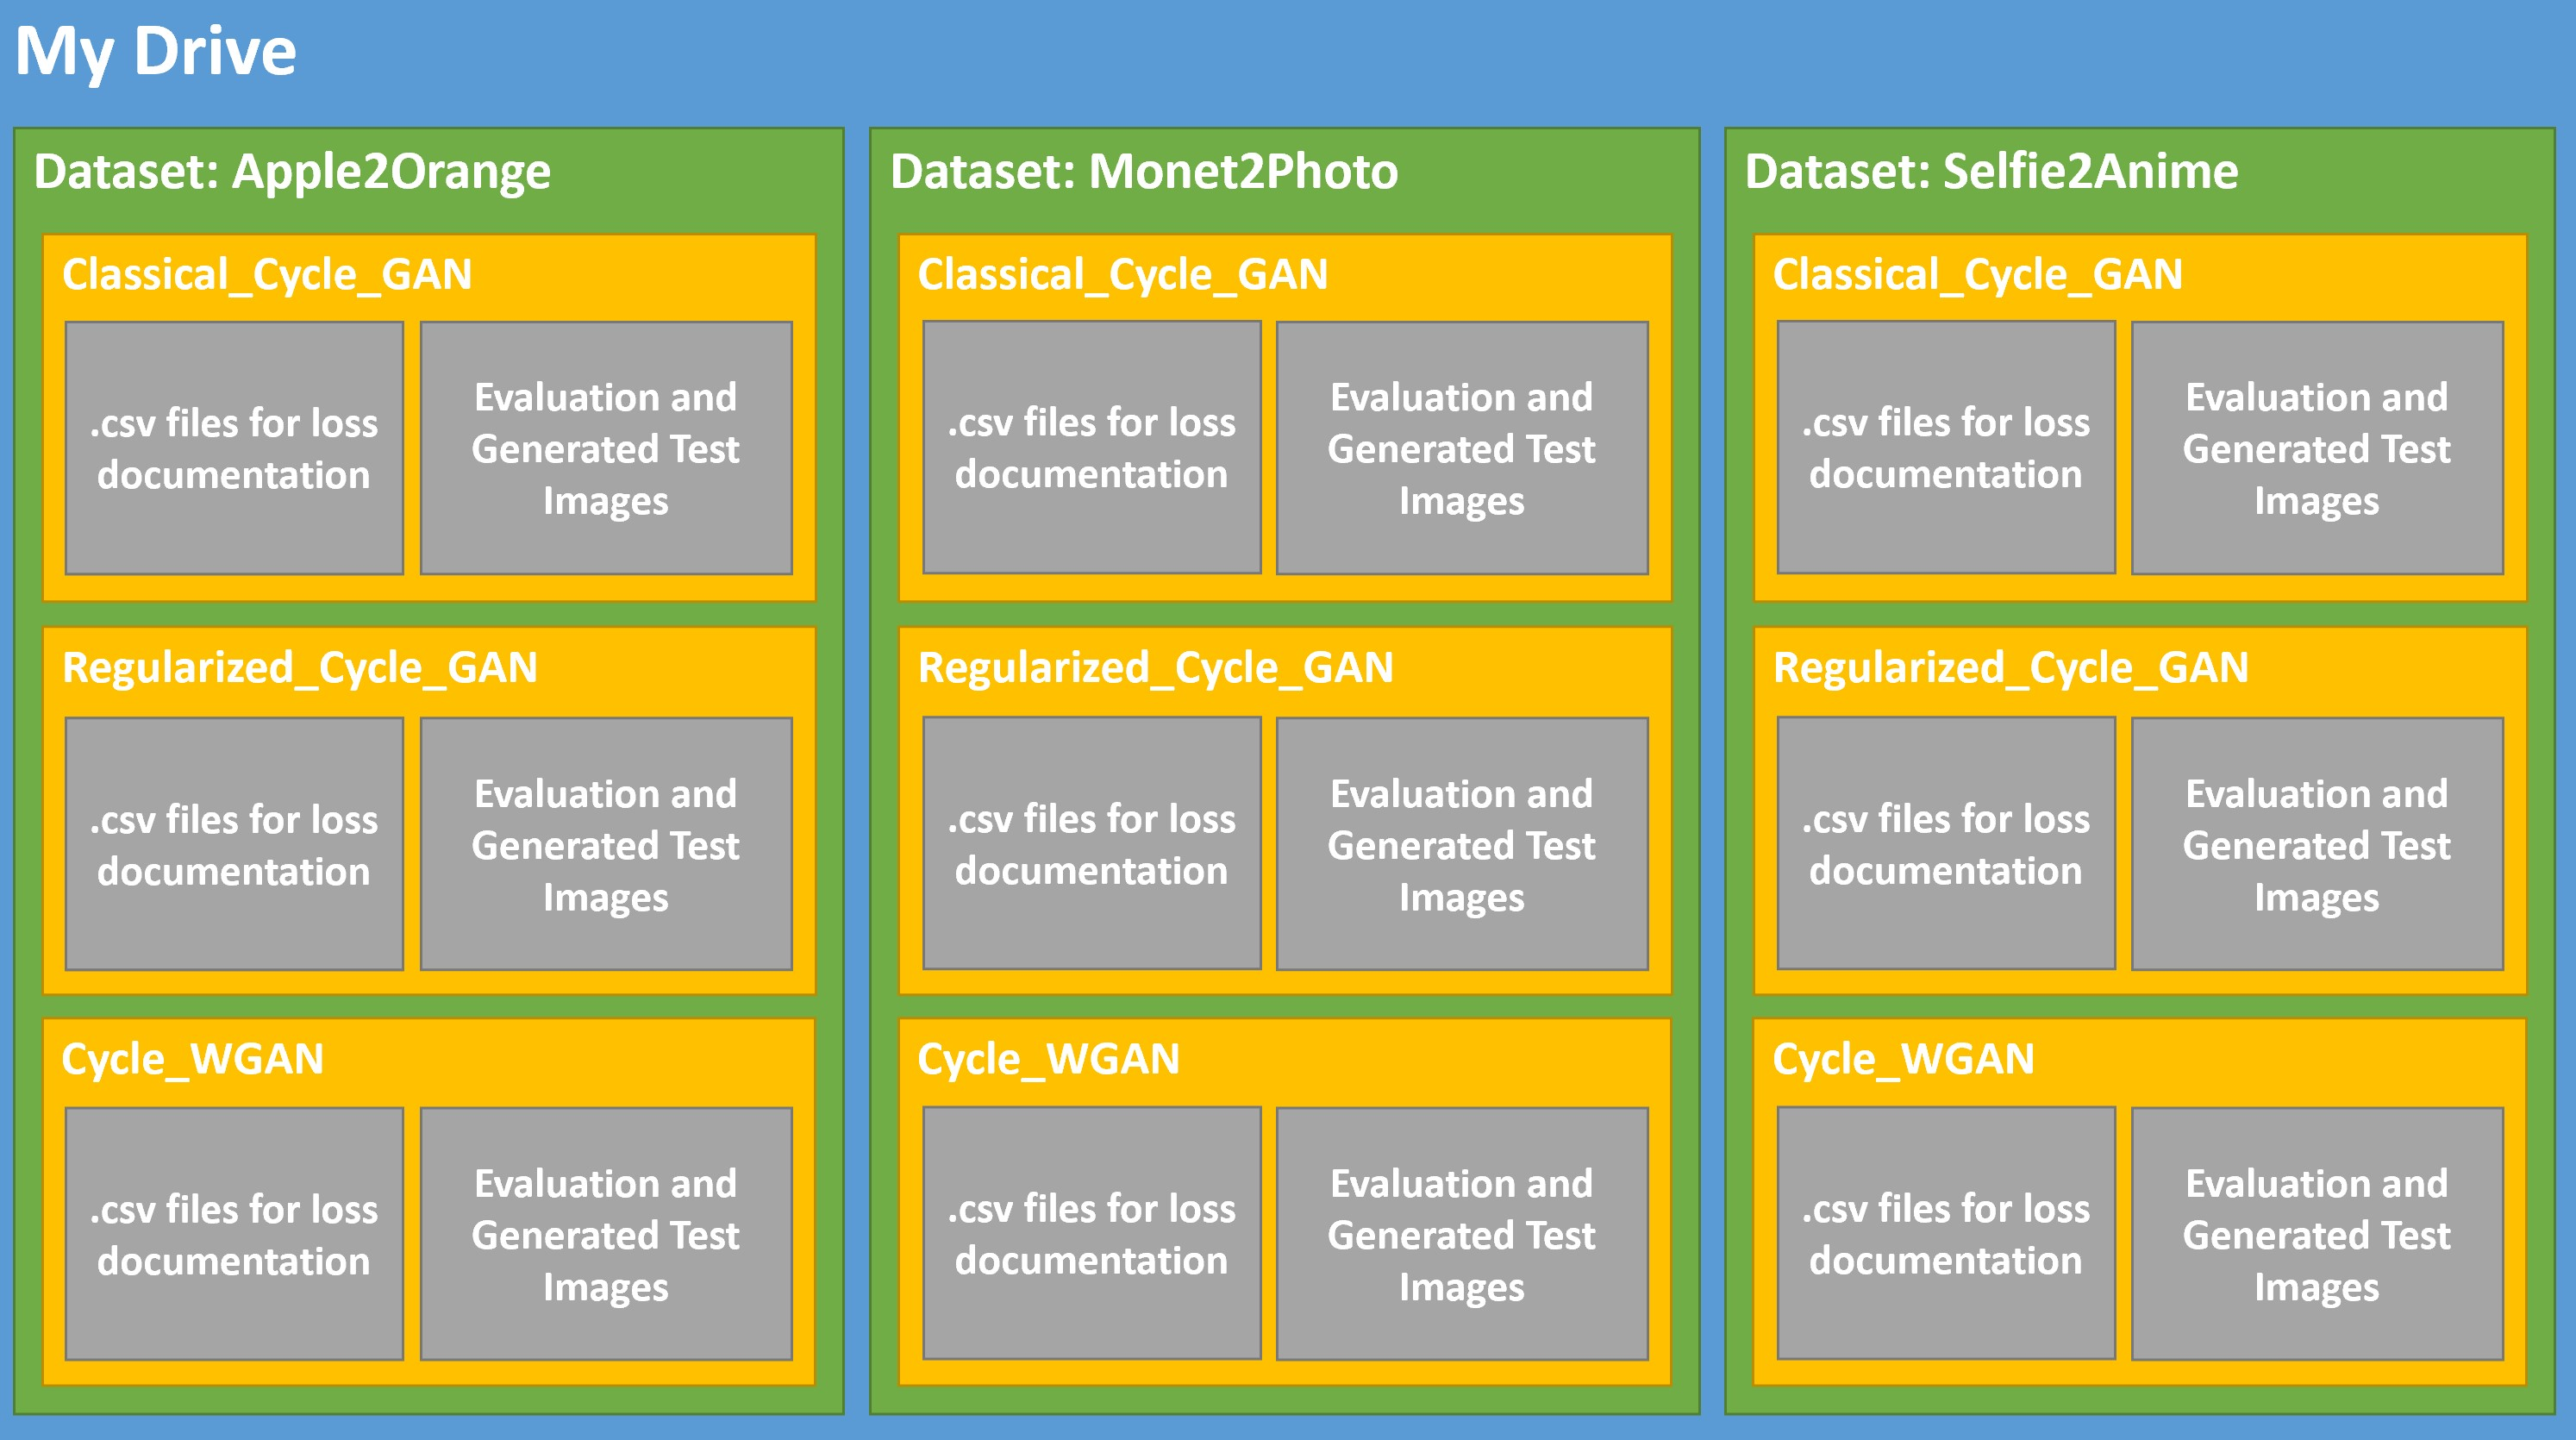
\includegraphics[width=\linewidth]{fileStructure}
	\caption{The folder structure to store the data in Google Drive.}
	\label{fig:fileStructure}
\end{figure}

%------------------------------------------------
\section{Variations of the Cycle\ac{GAN}}
After the pure reimplementation of the Cycle\ac{GAN}, two further improvements are implemented. All three variants are then compared with each other. The implementation of the two improved variants is explained in more detail in the following two subsections.

\subsection{Regularized Cycle GAN}
The first idea is taken from the original paper, see \cite{image-to-image-ccan}, and continued. Here, the Cycle\ac{GAN} was already tested with options for regularization. In this variant a further class for the \ac{ResNet} block, the \texttt{Regularized\_ResNet\_Block}, is programmed. This contains an additional dropout layer after the first convolutional layer. The dropout rate is assumed to be $0.5$.

Since the code should be written lean and collected in one colab notebook, the generator class is passed another argument at initialization, the \texttt{Regularized\_Cycle\_GAN}. If this argument is set to \textit{false}, then the default \ac{ResNet} is used during initialization. Is this argument set to \textit{true} during initialization, the Cycle\ac{GAN} is built with regularized \ac{ResNet} blocks.

Beside the adjustment of the \ac{ResNet} blocks in the generator, also the discriminator is adjusted. Already when initializing an instance of the discriminator class, the argument \texttt{kernel\_regularizer} with a L2 regularization loss is introduced to the convolutional layers. In the standard version of the Cycle\ac{GAN} this is also initialized, but not used. Therefore, the argument \texttt{Regularized\_Cycle\_GAN} is passed to the training step of the discriminator to control the computation of the loss dependent on it. If the argument is set to \textit{true}, the L2 loss for the discriminator is added and used for backpropagation.


\subsection{Cycle Wasserstein\ac{GAN}}
Furthermore, another method is introduced, according to \cite{wgan-improvement}. Here, instead of proceeding according to a simple \ac{GAN}, this is replaced by a \ac{WGAN}. This leads to the fact that first of all instead of the optimizer \textit{Adam}, the optimizer \textit{\ac{RMSProp}} is used. In addition, the weights in the discriminator are clipped, which also leads to the fact that the discriminator now has to be trained five times more than the generator. Furthermore, the \textit{sigmoid} activation is removed from the output layer of the discriminator. To implement all of this, a new class, \texttt{Cycle\_WGAN\_Discriminator}, is programmed for the \ac{WGAN} discriminator.

So that the network can also be included in the same lean colab notebook, the argument \texttt{Cycle\_WGAN} is introduced. If the argument is set to \textit{true}, then a Cycle-\ac{WGAN} is created, in the other case a standard Cycle\ac{GAN}. Here then also the optimizer is initialized instead of as \textit{Adam}, as \textit{\ac{RMSProp}}.

%------------------------------------------------

\section{Results and Analysis}
In this section, the results are presented and an analysis of the results is carried out. Since not all results can be presented here, only selected analyses are presented as examples. All other analysis data can be viewed in the associated Github reposistory~\cite{ourGithubRepo}.

\subsection{Training and Test performance}
\autoref{fig:trainTestComparisonAppl2orange} shows a graph including the averaged training and test losses of the two discriminator and two generator types. In general the discriminator losses are about 30 to 40\% smaller than the generator losses. Both types show a decreasing trend of the losses, whereby this is more evident for the generator losses than for the discriminator losses. This may also be due to the fact that the discriminator losses start out significantly smaller. Furthermore, it can be seen that the test losses for both discriminators fluctuate significantly more than the training losses, whereas this is exactly the opposite for the generators. At the end of the 2700 training steps (3 epochs), the generators training losses and the discriminator B test loss have a decreasing trend, while all the others have a slightly increasing trend. However, since the trend is downward over the entire 3 epochs, these slightly increasing trends will probably only lead to local maxima in further training.

\begin{figure}[htb] 
	\centering 
	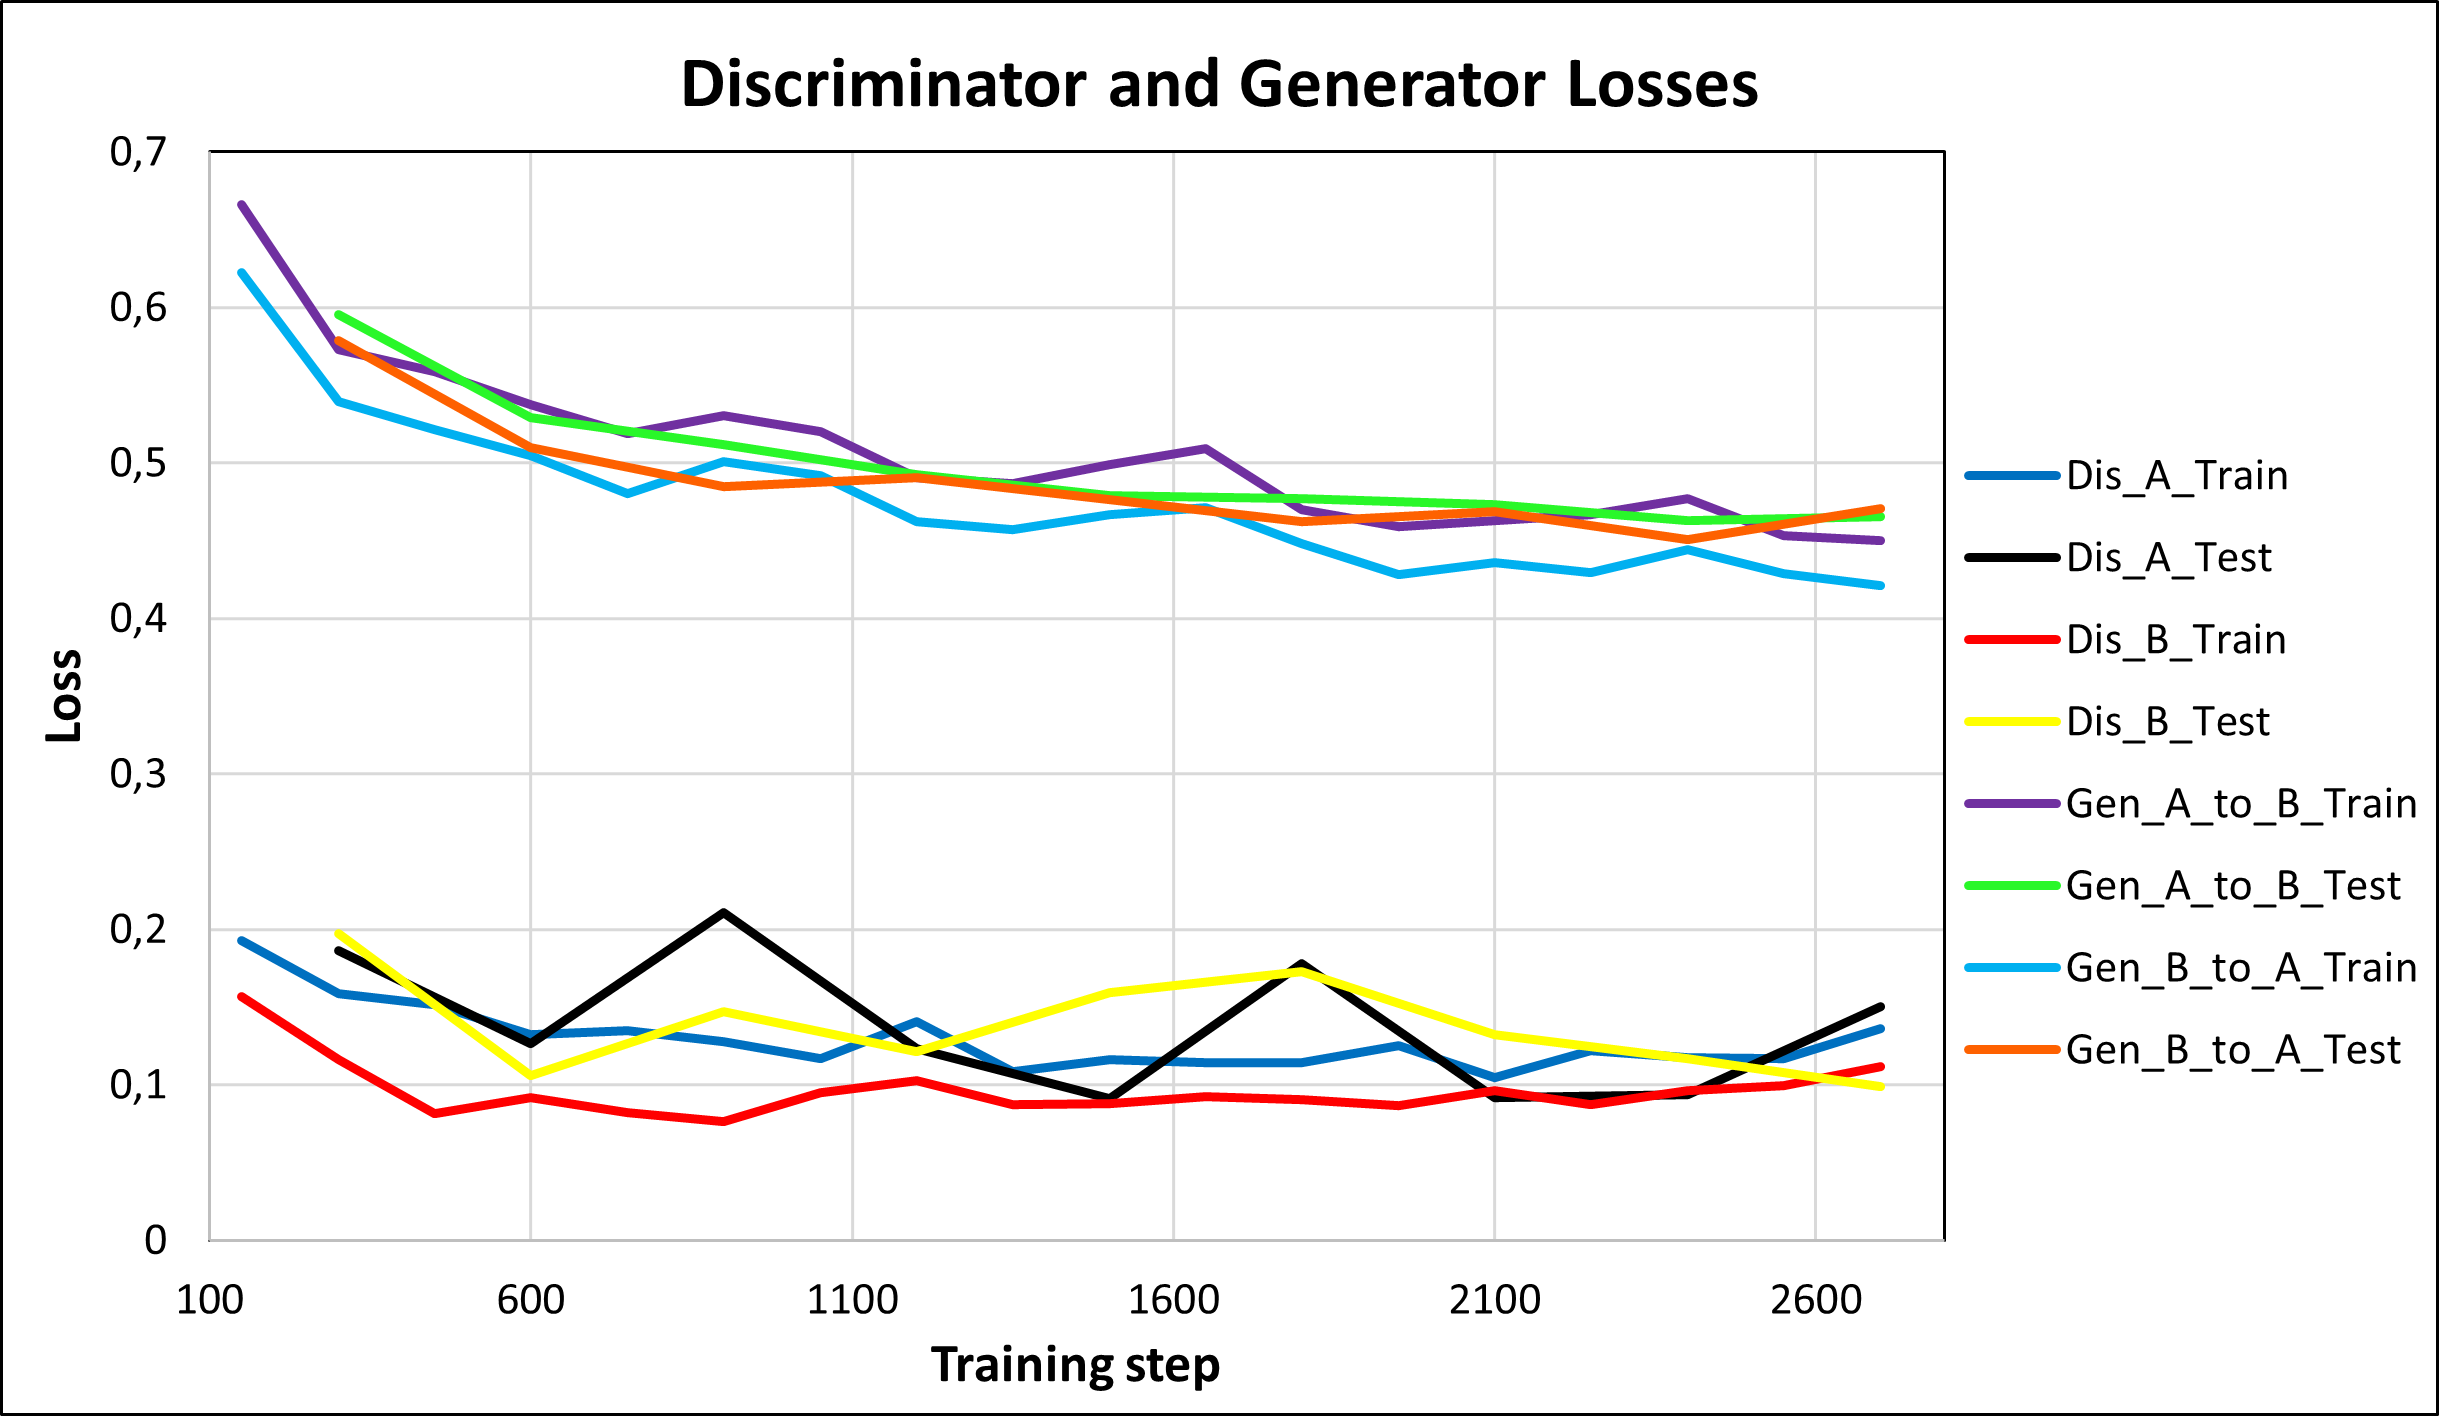
\includegraphics[width=\linewidth]{trainTestComparisonAppl2orange}
	\caption{History of discriminators and generator losses for test and training data over the training epochs of the dataset \textit{apple2orange}.}
	\label{fig:trainTestComparisonAppl2orange}
\end{figure}

Overall, however, it can be said that training and test losses run in tandem with each other and show a tendency to improve the network architecture with the implementation of the training.

For dataset \textit{monet2photo}, the overall discriminator losses are also lower than those of the generators. Furthermore, falling trends can be seen here as well. In contrast to dataset \textit{apple2orange}, the discriminator test and training losses diverge more. Overall, the generator losses are also about 10\% smaller than those of dataset \textit{apple2orange}.

\subsection{Components of the Generator loss}
Another interesting point of analysis is the examination of the various losses of the generator presented earlier. For dataset \textit{monet2photo}, these are seen from \texttt{generator\_A\_to\_B} in \autoref{fig:componentsGeneratorLossMonet2Photo}. As can be seen, the losses are almost all on a downward trend. The adversarial loss is very striking. This has a very strong upward tendency after about 1200 training steps. Despite all this, the combined loss of the generator (weighted overall loss) maintains the downward trend. Towards the end, the adversarial loss begins to indicate a downward trend again. Nevertheless, there is currently a global maximum at training step 2550.

\begin{figure}[htb] 
	\centering 
	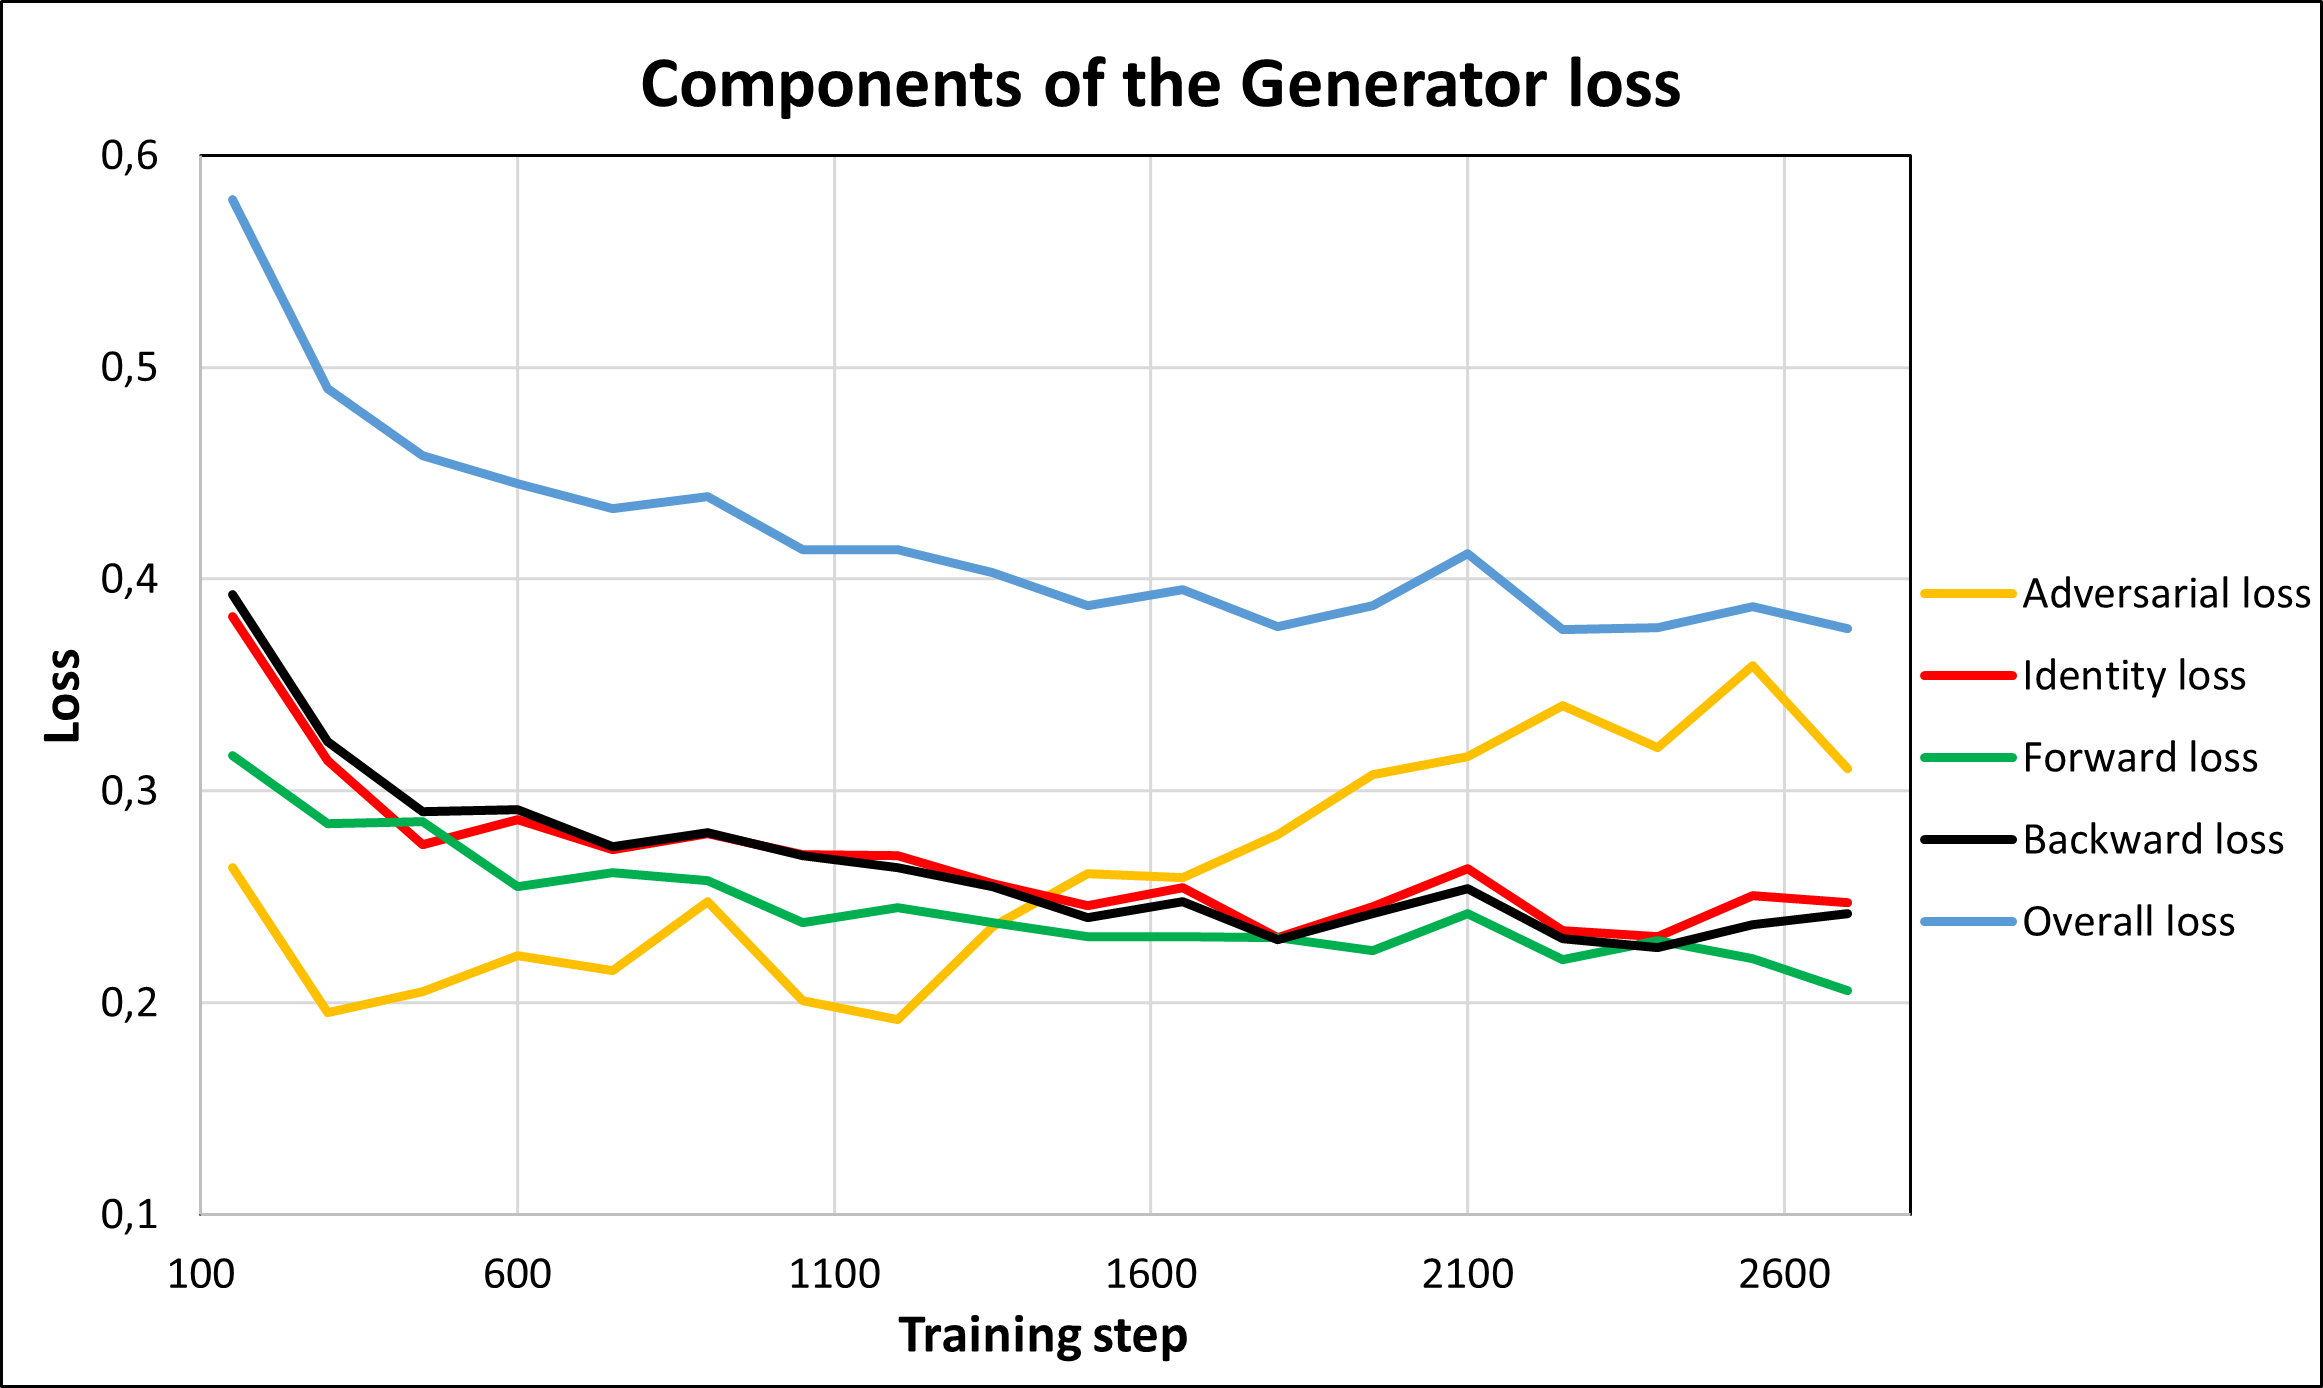
\includegraphics[width=\linewidth]{componentsGeneratorLossMonet2Photo}
	\caption{History of the different generator losses (\texttt{generator\_A\_to\_B}) of the training data over all trainings epochs of the dataset \textit{monet2photo}.}
	\label{fig:componentsGeneratorLossMonet2Photo}
\end{figure}

The adversarial loss in \autoref{fig:componentsGeneratorLossMonet2Photo}, however, never exceeds the value of the weighted overall loss, as is the case with dataset \textit{apple2orange}. But here too, despite all this, the other losses show a clear downward trend. Accordingly, it can be said that here too it is clear that the network improves over the course of the training.

\subsection{Comparison of the Cycle\ac{GAN} variations}
The different Cycle\ac{GAN} variations show different progressions in the losses, see \autoref{fig:generatorCycleGANTypes} and \autoref{fig:discriminatorCycleGANTypes}. While the discriminator losses show only a very slight downward trend within the three epochs, this trend can be seen more clearly in the generator losses. While the curve for the Cycle\ac{WGAN} generator loss is much smoother, it is much more erratic for the discriminator than for the other variations. The lowest generator loss is achieved by the classic Cycle\ac{GAN}, whereas this is not the case with the discriminator. This may also be related to the fact that better generated images are also more difficult to detect by a discriminator and vice versa. On the basis of these results, it is not possible to say whether one of the networks works better or worse than another. For this, an even longer training period would provide more information. 

\begin{figure}[htb] 
	\centering 
	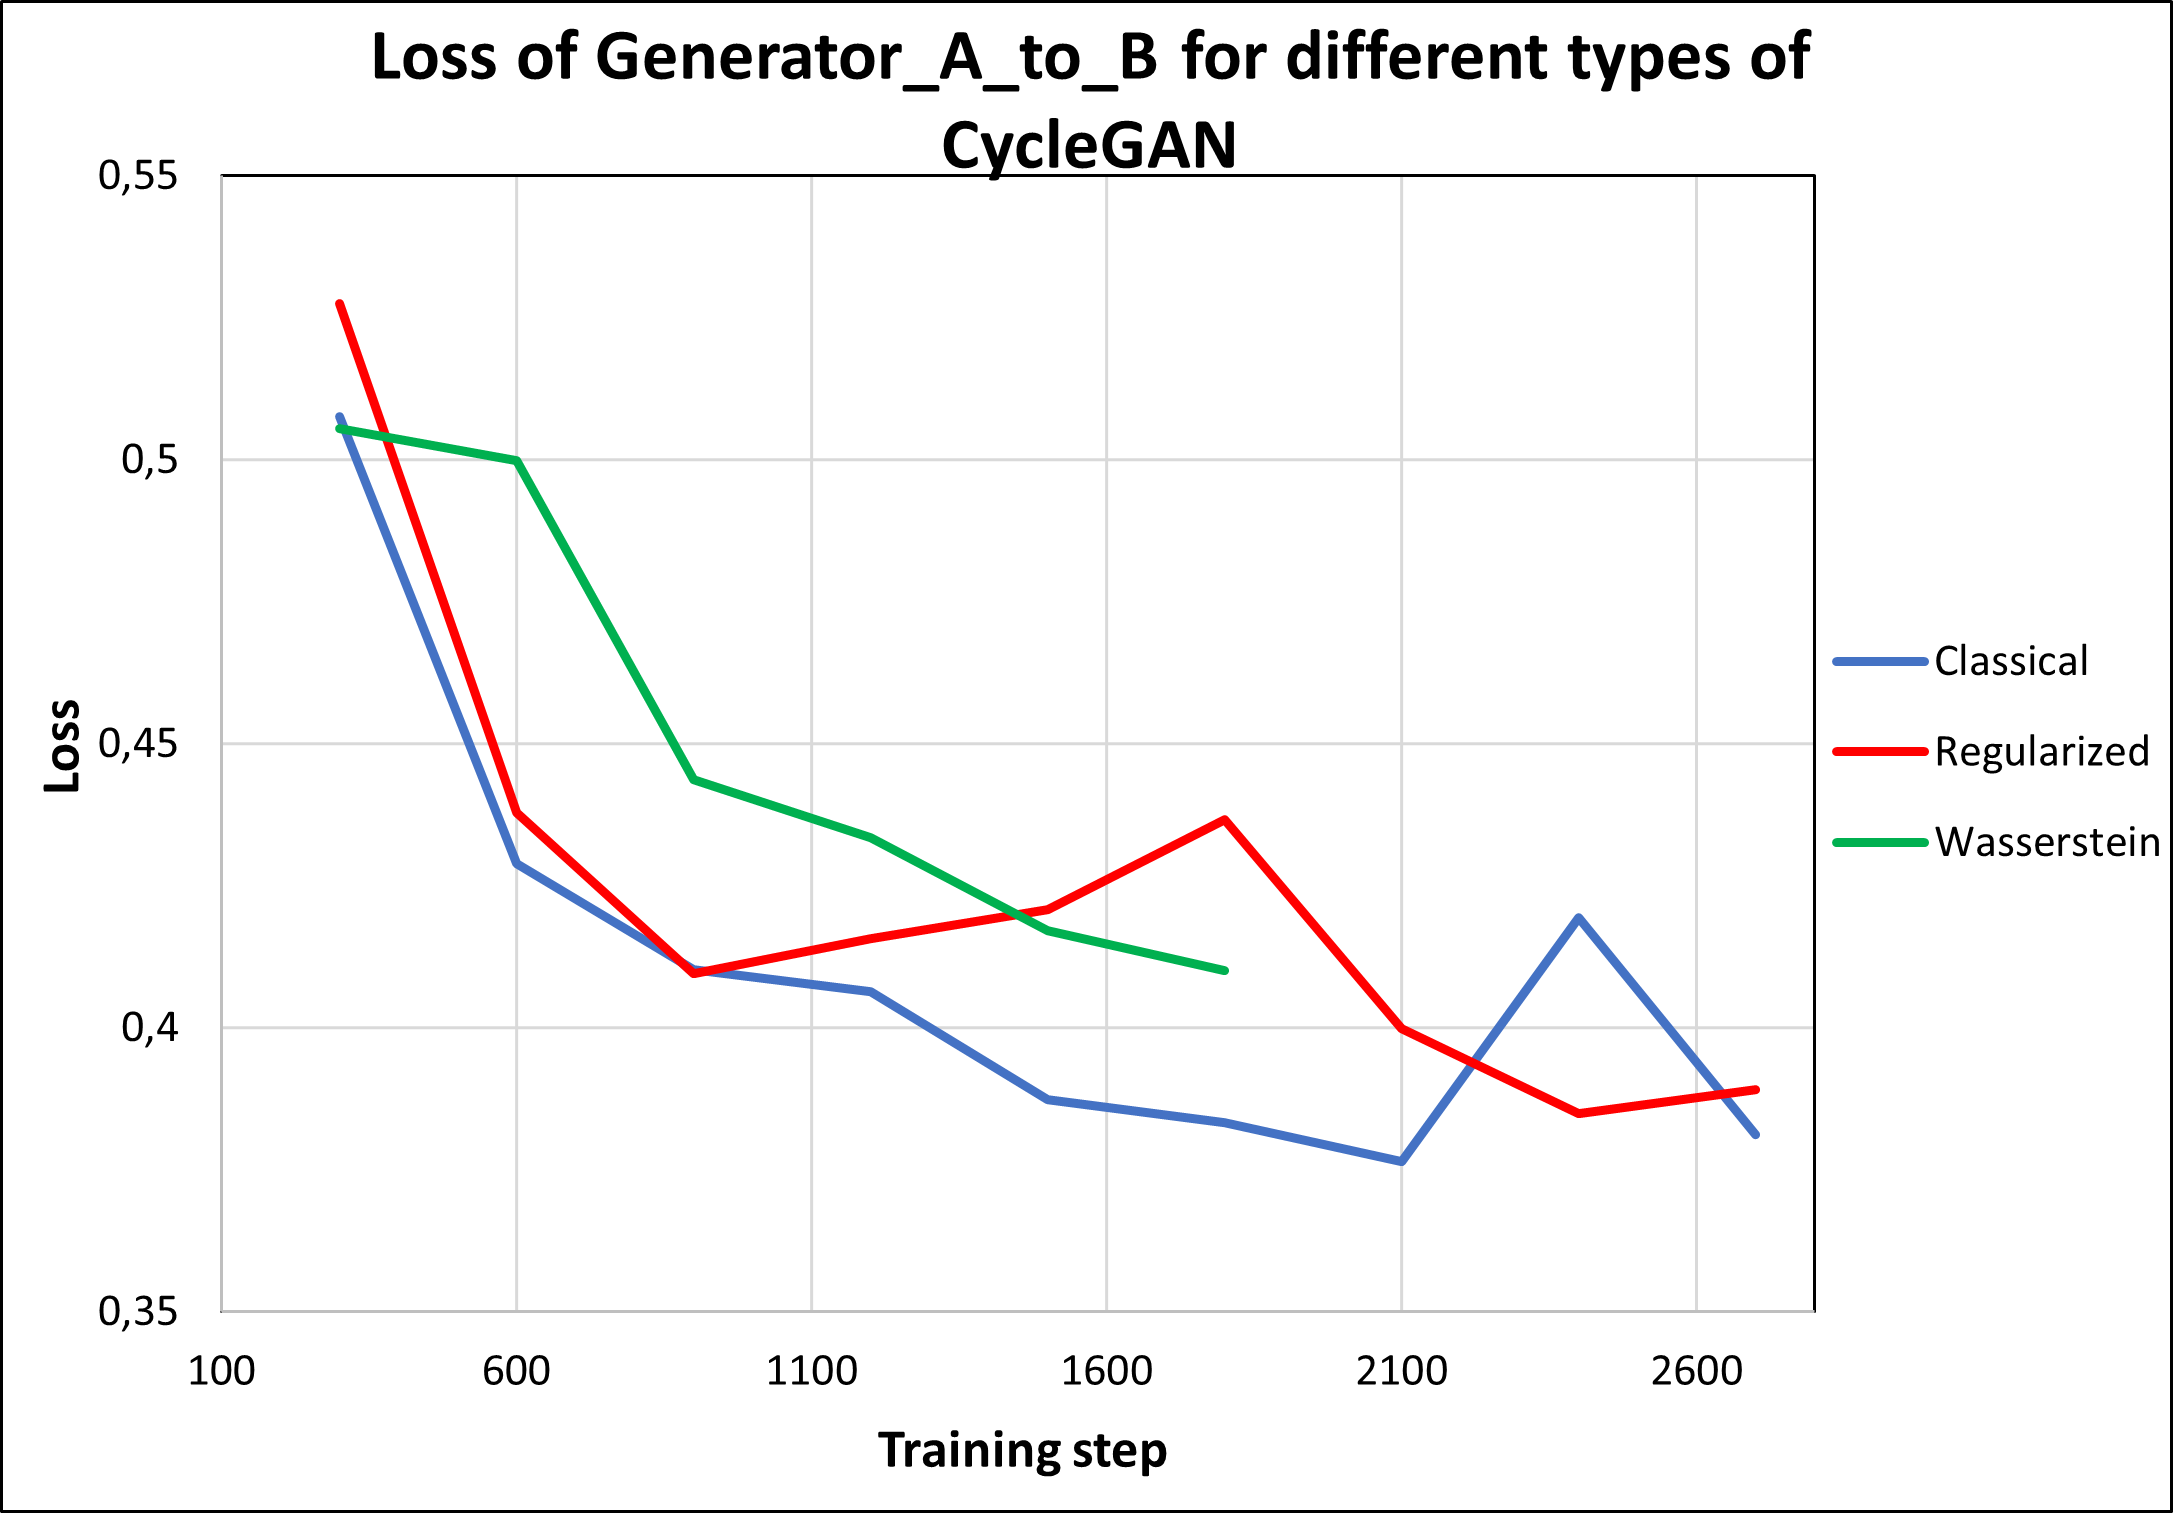
\includegraphics[width=\linewidth]{generatorCycleGANTypes}
	\caption{History of the overall loss of different Cycle\ac{GAN} variations of (\texttt{generator\_A\_to\_B}) of the training data over all trainings epochs of the dataset \textit{monet2photo}.}
	\label{fig:generatorCycleGANTypes}
\end{figure}

\begin{figure}[htb] 
	\centering 
	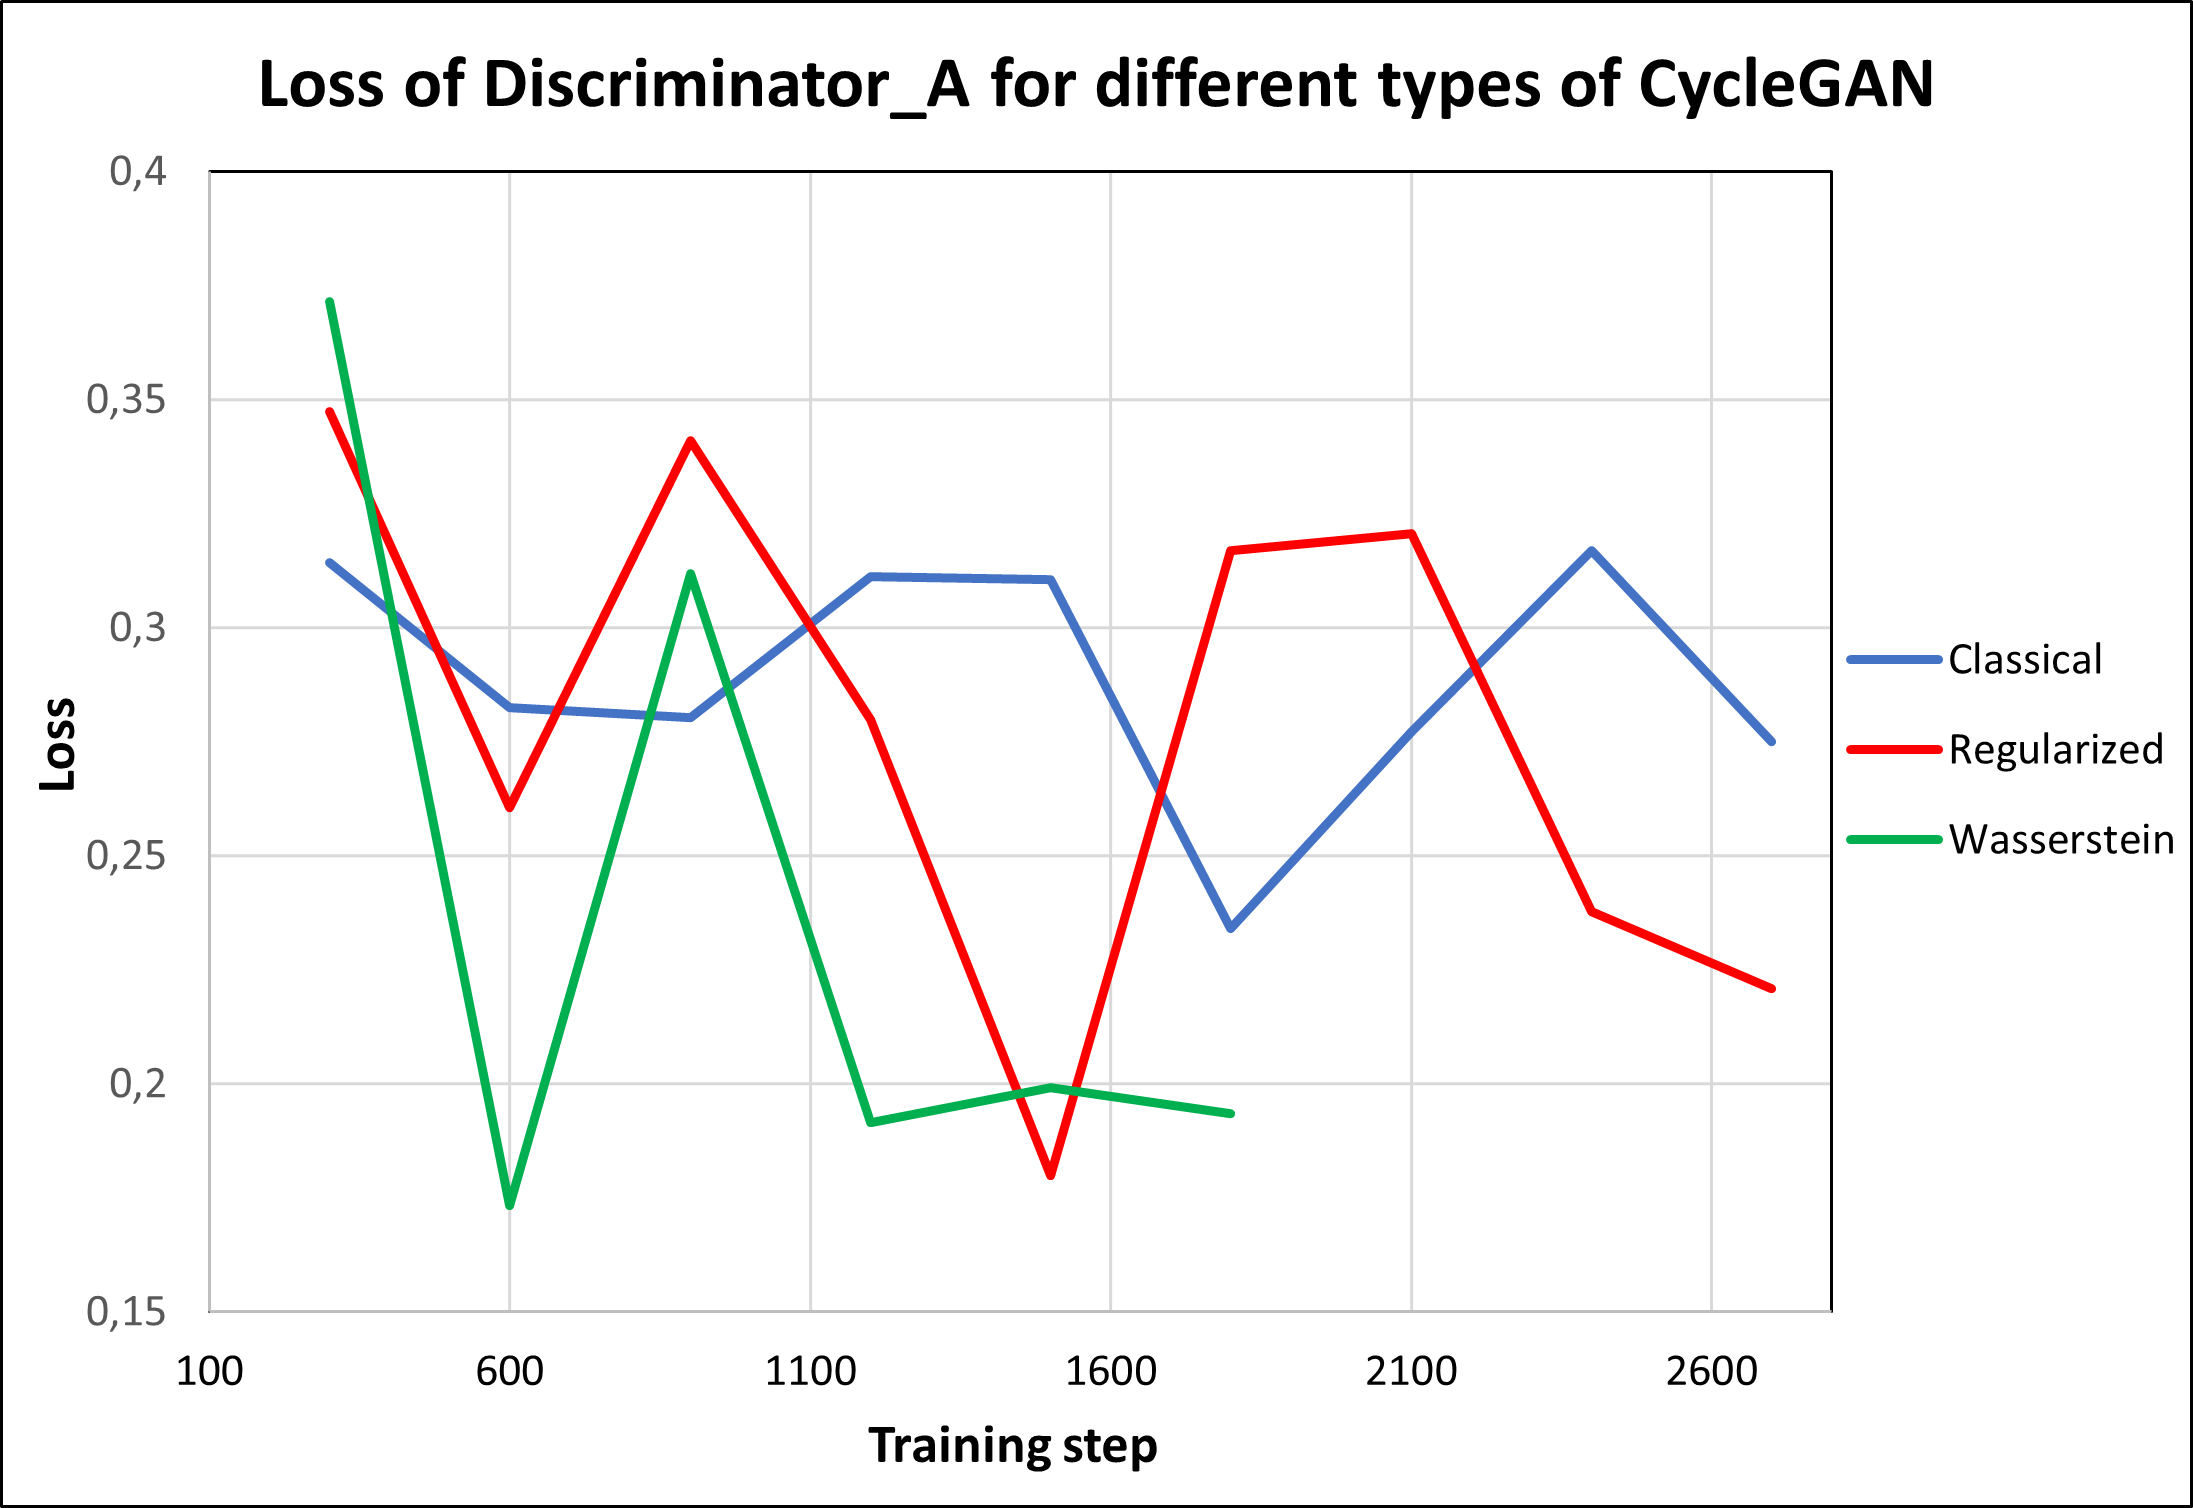
\includegraphics[width=\linewidth]{discriminatorCycleGANTypes}
	\caption{History of the overall loss of different Cycle\ac{GAN} variations of (\texttt{discriminator\_A}) of the training data over all trainings epochs of the dataset \textit{monet2photo}.}
	\label{fig:discriminatorCycleGANTypes}
\end{figure}

Another possibility is to compare the quality of the sample images. \autoref{fig:ClassicalCycleGANExample} shows an already great success after three epochs in the translation of an apple image into an orange image. In comparison, the generated images of the other variations, see \autoref{fig:CycleWGANExample} and \autoref{fig:RegularizedCycleGANExample}, look much less like oranges. However, no qualitative statement can be made about whether the generated image of the Regularised Cycle\ac{GAN} or Cylce{WGAN} looks more realistic than the other. Both images are very similar although the losses differ in numbers.
You can see the transitions between the individual fruits quite well despite the generated images. The borders were not changed much by any of the Cycle\ac{GAN} variants. This shows that all Cycle\ac{GAN} variations have basically recognised the fruit feature as such.

\begin{figure}[htb] 
	\centering 
\begin{subfigure}[b]{0.45\linewidth}
	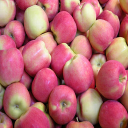
\includegraphics[width=\linewidth]{ClassicalCycleGANOriginalDomainA}
	\caption{Original example image of domain A}
\end{subfigure}
\hfill
\begin{subfigure}[b]{0.45\linewidth}
	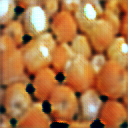
\includegraphics[width=\linewidth]{ClassicalCycleGANGenDomainBAfter8}
	\caption{Generic image after 2700 training steps}
	\end{subfigure}
\caption{Example of an image processed by the Classical Cycle\ac{GAN} from domain A to B of dataset \textit{apple2orange}}
\label{fig:ClassicalCycleGANExample}
\end{figure}

\begin{figure}[htb] 
	\centering 
\begin{subfigure}[b]{0.45\linewidth}
	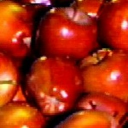
\includegraphics[width=\linewidth]{CycleWGANOriginalDomainA}
	\caption{Original example image of domain A}
\end{subfigure}
\hfill
\begin{subfigure}[b]{0.45\linewidth}
	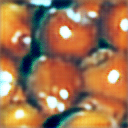
\includegraphics[width=\linewidth]{CycleWGANGenDomainBAfter5}
	\caption{Generic image after 1500 training steps}
	\end{subfigure}
\caption{Example of an image processed by the Cycle\ac{WGAN} from domain A to B of dataset \textit{apple2orange}}
\label{fig:CycleWGANExample}
\end{figure}

\begin{figure}[htb] 
	\centering 
\begin{subfigure}[b]{0.45\linewidth}
	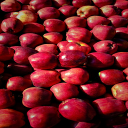
\includegraphics[width=\linewidth]{RegularizedCycleGANOriginalDomainA}
	\caption{Original example image of domain A}
\end{subfigure}
\hfill
\begin{subfigure}[b]{0.45\linewidth}
	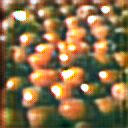
\includegraphics[width=\linewidth]{RegularizedCycleGANGenDomainBAfter8}
	\caption{Generic image after 2700 training steps}
	\end{subfigure}
\caption{Example of an image processed by the Regularized Cycle\ac{GAN} from domain A to B of dataset \textit{apple2orange}}
\label{fig:RegularizedCycleGANExample}
\end{figure}

\subsection{Limitations of the Cycle\ac{GAN} architecture}
As the training of the \textit{selfie2anime} dataset takes too long for this project framework, only very few training steps (300) could be carried out and only one test could be conducted after them. The result is shown in \autoref{fig:CycleWGANSelfieExample}. You can see that the colours are transformed well and quickly, whereas the contours are not. This can be seen very clearly in the area of the eyes, for example.

This result is also reflected in the comparison with the \textit{apple2orange} example, where the colour of the apples changes quite quickly to orange, but the contours remain almost untouched.

\begin{figure}[htb] 
	\centering 
\begin{subfigure}[b]{0.45\linewidth}
	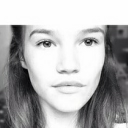
\includegraphics[width=\linewidth]{RegularizedCycleGANOriginalSelfieDomainA}
	\caption{Original example image of domain A}
\end{subfigure}
\hfill
\begin{subfigure}[b]{0.45\linewidth}
	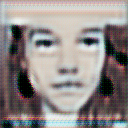
\includegraphics[width=\linewidth]{RegularizedCycleGANGenAnimeDomainB}
	\caption{Generic image after 300 training steps}
	\end{subfigure}
\caption{Example of an image processed by the Regularized Cycle\ac{GAN} from domain A to B of dataset \textit{selfie2anime}}
\label{fig:CycleWGANSelfieExample}
\end{figure}


\section{Conclusion and Future work}
The analysis between different datasets, as well as a more detailed look at the losses between each other, and much more could be explored in more detail. However, this is outside the time frame of the project. Further limits and extension ideas are touched on below.

Unlike previously planned, the analysis could only be carried out more detailed using the Tensorflow datasets, as the duration of the training process for the Kaggle dataset \textit{selfie2anime} was too long. Despite a subsequent reduction of the epochs to one, the network needed more than half a day. In addition, with Goolge Colab's limitation of GPU time, it was hardly possible to train over such a long period. Nevertheless, few results of the first training steps were stored in the repository. However, since this is difficult to compare with the other datasets due to the few trainings steps in comparison, a more detailed analysis was not performed here. However, since a few interesting features already developed within the first training steps, this analysis should be expanded in further projects.

The images of the datasets also had to be greatly reduced in size in order to be able to train approximately within the framework of the project. The behaviour of the network at a higher resolution of the images is another interesting detail to investigate.

Furthermore, it would be possible to expand the training and tests. In order to have an even better comparability between the Cycle\ac{GAN} variations, the same 5 test images could always be used for all variations. This was only noticed during the analysis and was no longer implemented due to time constraints, among other things. Another difficulty for the implementation is also the design of the notebook, as this is always executed anew. The five test images would therefore have to be administered externally beforehand in order to be able to guarantee access to the always same images.

Another improvement can be found in the saving of data. Here, an even more detailed evaluation could take place if data were saved after each training step. However, due to the huge flood of data and the increased computing time, this was not done.

In summary, the results of the project are more meaningful than previously expected. Nevertheless, there is much more potential of the Cycle\ac{GAN}s that could not be realised in this project due to time constraints.


%----------------------------------------------------------------------------------------
%	REFERENCE LIST
%----------------------------------------------------------------------------------------

\phantomsection
\bibliographystyle{unsrt}
\bibliography{sample}

%----------------------------------------------------------------------------------------

\begin{acronym}
\acro{BAIR}[BAIR]{Berkeley AI Research}
\acro{IANNWTF}[IANNWTF]{Implementing Artificial Networks with Tensorflow}
\acro{GAN}[GAN]{Generative Adversarial Network}
\acro{ReLu}[ReLu]{Rectified Linear Units}
\acro{ResNet}[ResNet]{Residual Network}
\acroplural{ResNet}[ResNet]{Residual Networks}
\acro{RMSProp}[RMSProp]{Root Mean Squared Propagation}
\acro{WGAN}[WGAN]{Wasserstein \ac{GAN}}
%\acroplural{Kuerzel}[Kurzform des Plurals]{Langform des Plurals}
\end{acronym}

%----------------------------------------------------------------------------------------


\end{document}